Dans un système ayant un seul PONE et un seul TARE (en plus du revendeur, du marché de gros et de l'AMI), le client demande une quantité d'énergie qui n'est pas disponible pour le moment ... Par contre, au bout de quelques instants de fonctionnement, la demande du client peut-être satisfaite (car le PONE a suffisamment fourni d'énergie). Cela est possible après une nouvelle demande cu client.

Pour ce scénario, nous avons réalisé une demande du client sur une énergie de type "Electricité" avec aucune restriction sur le type d'électricité demandé avec une quantité de 100. La première fois cela échouera, mais après un petit moment, la requête sera satisfaite.

\begin{figure}[h]
    \centering
    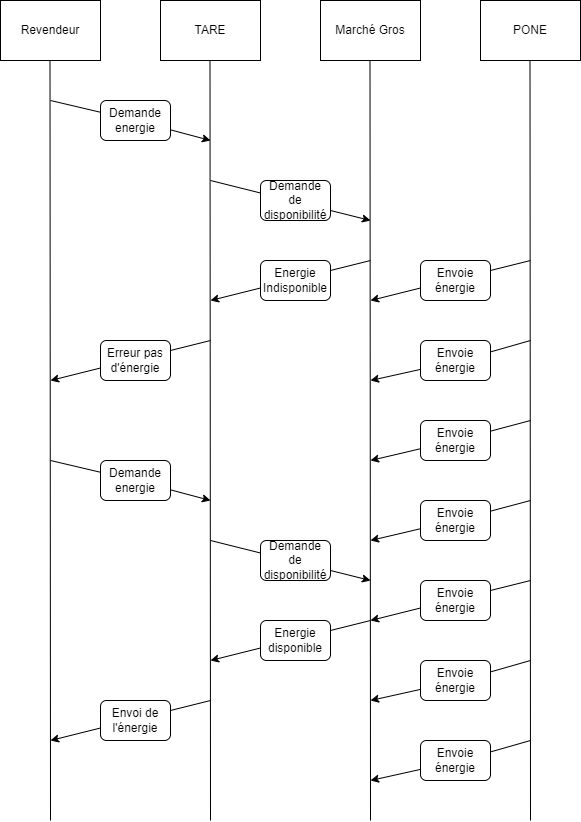
\includegraphics[width=110mm, height=150mm]{images/ScenarioB.png}
    \caption{Schéma du scénario B}
    \label{img:mesh23}
\end{figure}
\newpage